% Background Chapter

\chapter{Literature review} % Chapter Title
\label{ch_LitRev}

\section{What are Volatile Organic Compounds (VOCs)?}
\label{ch_LitRev:sec:what_are_vocs}
  \subsection{VOCs}
    Organic compounds are members of a large class of chemicals whose molecules contain carbon, with the exception of a few compounds such as carbides, carbonates (CO$_3$), and simple oxides of carbon and cyanides.
    Organic compounds can be categorised based on their vapour pressure, which is the tendency of a liquid or solid to vaporise.
    Compounds with high vapour pressures at standard temperature are classed as volatile, and have a felicity to evaporate at low temperatures.
    Plants contain tens of thousands of organic compounds, it's likely that fewer than 40 are emitted due to the low volatility of most of them \citep{Guenther2000}.
    
    Atmospheric organic compounds are legion and differ by orders of magnitude with respect to their fundamental properties, such as volatility, reactivity, and cloud droplet formation propensity.
    VOCs have vapour pressure greater than $10^{-5}$~atm, and are mostly generated naturally by plants, which emit around 1000~Tg per year \citep{Guenther1995, Glasius2016}.
    Due to their high volatility these compounds are generally seen in the gas phase.
    Organic compounds with a lower volatility are classed as semi-volatile (SVOCs: vapour pressure between $10^{-5}$ and $10^{-11}$~atm) are seen in both gas and particle phase depending on temperature and pressure.
    Organic compounds with even lower vapour pressure are generally found in the particle phase in aerosol particulate matter \citep{Glasius2016}.

    VOC emissions result in radical cycling, acid deposition, and the production of tropospheric ozone, and secondary aerosols \citep{Atkinson2000}.
    These have impacts on climate (through radiative forcing) and air quality, affecting both human health and crop yields \citep{IPCC_Chapter2, Avnery2011, Lelieveld2015}.
    Understanding the drivers of trends in biogenic volatile organic compound emissions (BVOCs) is needed in order to estimate future carbon fluxes, changes in the water cycle, air quality, and other climate responses \citep{Yue2015}.
    
    In the 1990's, the World Meteorological Organisation (WMO) estimated that we are emitting 360~Mt yr$^{-1}$ of methane (CH$_4$), one of the more abundant and potent VOCs, while biogenic emissions were around 200~Mt yr$^{-1}$ \citep{Atkinson2000}.
    At that point in time, emissions of other VOCs (Non Methane VOCs - NMVOCs) were estimated at 1150~Mt yr$^{-1}$ (of carbon) from biogenic sources, and 100~Mt yr$^{-1}$ from anthropogenic sources \citep{Guenther1995, Atkinson2000}.
    These estimates were based on the Model of Emissions of Gases and Aerosols from Nature (MEGAN, \citet{Guenther1995}).
    
    MEGAN initially included a simple canopy radiative transfer model, which parameterised sun-lit and shaded conditions through a canopy.
    Early models didn't account for abiotic stresses, such as drought, prior rainfall and development processes, although these influenced species specific emissions by more than an order of magnitude \citep{Niinemets2000}.
    Isoprene emissions were based on temperature, leaf area, and light, but have since been updated to include leaf age activity \citep{Guenther1999}, and a leaf energy balance model \citep{Guenther2006} in MEGANv2.0.
    This update included a parameter for soil moisture, to account for drought conditions.
    
    MEGAN has recently been analysed using 30 years of meteorological reanalysis information by \citet{Sindelarova2014}.
    They estimate emissions of Biogenic VOCs (BVOCs) to be 760~Tg(C)yr$^{-1}$, 70\% (532~Tg(C)yr$^{-1}$) of which is isoprene.
    This is similar to isoprene emission estimates from MEGAN itself, of 400-600~Tg(C)yr$^{-1}$ \citep{Guenther2006}.
    
    MEGAN emissions estimates are termed bottom-up, as opposed to top-down which are derived from satellite measurements of the products of various VOCs.
    Using GOME satellite HCHO and a Beyesian inversion technique to derive isoprene emissions, \citet{Shim2005} estimated global isoprene emissions to be $\sim566$~TgC yr$^{-1}$. 
    This estimate is greater than initially thought and leads to decreased ($\sim10\%$) simulated OH concentrations to 9.5e5 molec cm$^{-3}$.
    
    Photolysis and oxidation of many VOCs initially form alkyl radicals ($\dot{R}$), and reactions with ozone (with alkenes or VOCs containing a double bonded carbon) lead to organic peroxy radicals (R$\dot{O}_2$). 
    These go on to form many prooducts and lead to (amongst other things) aerosol, formaldehyde, and ozone formation, depending on various other factors such as sunlight and NO pollution \citep{Atkinson2000}.
    
    VOCs are removed by wet and dry deposition, or transformed by reaction with OH, NO$_3$, or O$_3$,
    The process of deposition only accounts for a small fraction of the VOC loss, with the possible exception of the long lived methane compount \citep{AtkinsonArey2003}.
    Primary reductions occur through photolysis, OH oxidation, ozonolysis, and at night time in polluted areas, NO$_3$ \citep{AtkinsonArey2003, Brown2009}.
    In the presence of NO$_X = $ NO $+$ NO$_2$, non-methane organic compounds (NMOCs) and NMVOCs end up forming tropospheric ozone.
    This is achieved through photolysis of NO$_2$, concentrations of which are increased by NMOC and NO reactions \citep{AtkinsonArey2003}.
  
  \subsection{Hydroxyl (OH) and other radicals}
    \label{ch_LitRev:sec:RadicalFormation}
    
    The OH radical drives many processes in the atmosphere, especially during the day when photolysis of ozone drives OH concentrations \citep{Atkinson2000}.    
    OH is a key species which reacts with nearly all the organic compounds in the troposphere.
    The exceptions are chlorofluorocarbons (CFCs), and Halons not containing H atoms \citep{Atkinson2000}.
    OH and HO$_2$ concentrations largely determine the oxidative capacity of the atmosphere.
    Oxidation and photolysis are the two main processes through which VOCs are broken down into HCHO, O$_3$, CO$_2$ and various other species.
    
    Ozone is an important precursor to HO, as excited oxygen atoms (O(${}^1$D) are created through photolysis, which then go on to mix with water and form OH, as shown in this equation taken from \citet{Atkinson2000}:
    \begin{align*}
      O_3 + \text{hv}         & \to  O_2 + O({}^1D)   && (\lambda \le 335 \text{nm} \\%
      O({}^1D) + M            & \to  O({}^3P) + M     && (M=N_2, O_2)               \\%
      O({}^3P) + O_2 + M      & \to  O_3 + M          && (M=\text{air})             \\%
      O({}^1D) + H_2O         & \to  2OH              &&                            \\%
    \end{align*}
    This shows how some of the O$({}^1D)$ recycles back to Ozone, while some forms OH.
    NB: The wavelength was updated to 350~nm in \citet{AtkinsonArey2003}.
    
    In the late 90's it was understood that OH radicals are formed exclusively from photolysis of O$_3$, HONO, HCHO, and other carbonyls (R$_2$C=O) \citet{Atkinson2000}.
    TODO: Since then what do we know of OH formation?

    Nitrate radicals NO$_3$ are also largely formed through ozone reactions.
    They are photolysed very rapidly during they day, with a lifetime of about 5~s \citep{Atkinson2000}.
    If NO and O$_3$ are both in the atmosphere, the following reactions \citep{Atkinson2000} occur:
    \begin{align*}
      NO + O_3         & \to NO_2 + O_2      && \\%
      NO_2 + O_3       & \to NO_3 + O_2      && \\%
      NO_3 + \text{hv} & \to NO + O_2        && (\sim 10\%) \\%
      NO_3 + \text{hv} & \to NO_2 + O({}^3P) && (\sim 90\%) \\%
    \end{align*}
    A build up of NO$_3$ radicals can be seen at night, when the quick photolysis is not occurring \citep{Atkinson2000,Brown2009}.


  \subsection{Secondary Organic Aerosols}
    Fine particulate matter (PM$_{2.5}$) penetrates deep into the lungs and is detrimental to human health.
    Aerosols are suspended particulates and liquid compounds in the atmosphere, of which PM is an important subset.
    A substantial amount of PM is due to organic aerosols (OA) transforming in the troposphere leading to what's known as secondary organic aerosols (SOA) \citep{Kroll2008}.
    Formation of SOA is generally due to VOC oxidation and subsequent reactions \citep{Kanakidou2005}.
    In the \cite{Kanakidou2005} review of global SOA science, uncertainty in radiative forcing of aerosols is highlighted, and 20-90~\% of PM mass in the lower troposphere is OA.
    Less volatile OA also plays a role, although PM production from this source is complicated and makes up only a small fraction ($\sim1 %$) of the resulting PM \citep{Kroll2008,Bei2012}.
    
    One of the large uncertainties with OA is the total effect on radiative forcing, ten years ago it was well understood that most OA cool the atmosphere, with smaller particles having a larger affect due to the size matching the wavelengths of visible light \citep{Kanakidou2005}. 
    Transport and indirect effects complicate matters further, with cloud creation and modification of cloud properties being quite difficult to accurately predict.
    In the third IPCC report \citep{IPCC2001}, the uncertainty involved if OA forcing was a factor of 3 times the estimated effect. 
    This has since been improved however OA and cloud formation still remains a large uncertainty in more recent IPCC reports \citep{IPCC_Chapter2}.
    Image \ref{ch_LitRev:fig:IPCC_RF} shows the radiative forcings of various atmospheric constituents, it's clear that OA uncertainty dominates.
    
    \begin{figure}
      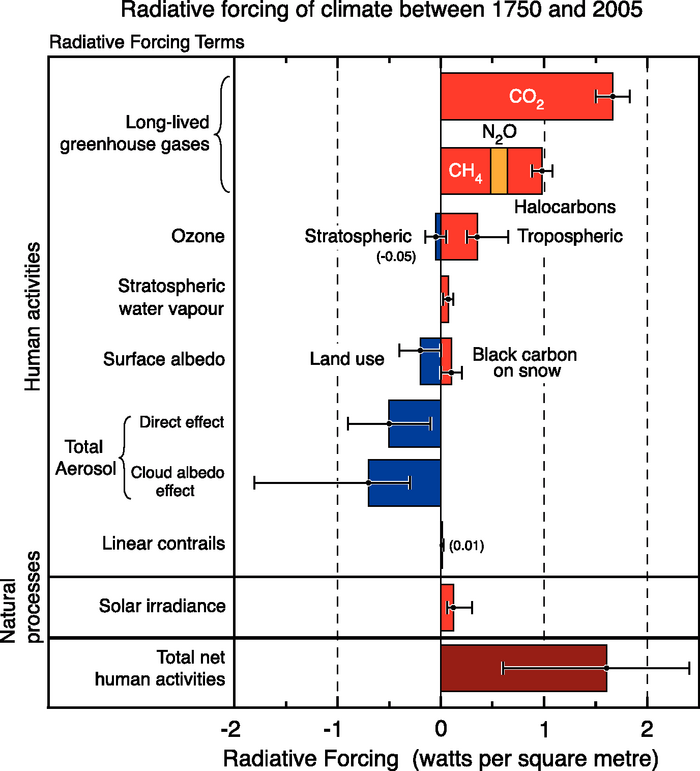
\includegraphics{Figures/AR4_RadiativeForcing.png}
      \caption{%
        The overall radiative forcings and uncertainties of several atmospheric constituents
	      This is an image taken from \cite{IPCC_Chapter2}, found at \url{https://www.ipcc.ch/publications_and_data/ar4/wg1/en/faq-2-1.html}.}
      \label{ch_LitRev:fig:IPCC_RF}
    \end{figure}
    
    (TODO: read more of Kanakidou2005)
  \subsection{Relationship with ozone}
    There is a complex relationship between NO$_X$, VOCs, and ozone, figure \ref{ch_LitRev:fig:NOXVOCOzone} shows this relationship over Houston, as modelled in \cite{Mazzuca2016}.
    Recently the relationship has been examined on the intradiel timescale showing that ozone production can be more or less sensitive to VOCs at different hours depending on location various other factors \citep{Mazzuca2016}.
    
    \begin{figure}
      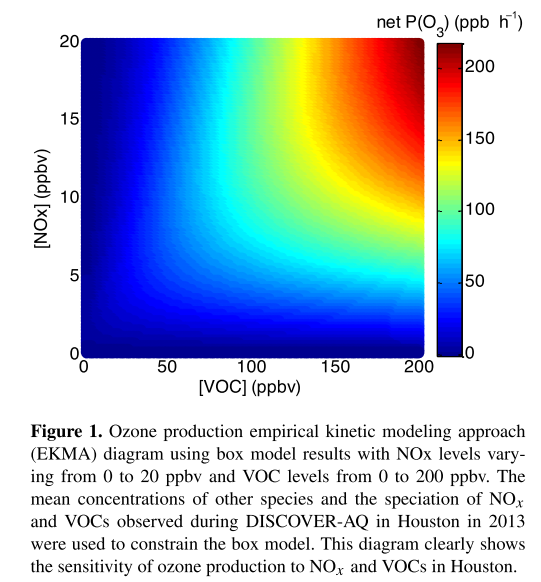
\includegraphics[width=.75\textwidth]{Figures/Mazzuca2016_NOxVOCOzone.png}
      \caption{Ozone production figure copied from \citet{Mazzuca2016}.}
      \label{ch_LitRev:fig:NOXVOCOzone}
    \end{figure}
    
    
%----------------------------------------------------------------------------------------
%	Natural gas and aerosol emission in Australia
%----------------------------------------------------------------------------------------
\section{Natural gas and aerosol emissions in Australia}
\label{ch_LitRev:sec:emissions}

  \subsection{Australia}

    Australia is largely covered by environments which are not heavily influenced by human activity.
    These regions are natural sources of the trace gases which make up less than 1\% of earth's atmosphere.
    Trace gases in the atmosphere can have a large impact on living conditions.
    They react in complex ways with other elements (anthropogenic and natural), affecting various ecosystems upon which life depends.
    Biogenic emissions affect surface pollution levels and can alter the radiative and particulate matter distribution of the atmosphere with harmful results.
    For example, ozone in the lower atmosphere is a serious hazard that causes health problems \citep{Hsieh2013}, damages agricultural crops worth billions of dollars \citep{Avnery2011}, and increases the rate of climate warming \citep{IPCC_2013_chap8}.
    Particulate matter in the atmosphere is also a major problem, causing an estimated 2-3 million deaths annually \citep{Hoek2013, Krewski2009, Silva2013, Lelieveld2015}. 

    Much of the landscape outside of urban areas is undeveloped and sparsely inhabited.
    In Australia most long term air quality measurements are performed in or near large cities.
    However, estimates of atmospheric gas and particulate densities, and their distributions over much of the continent are uncertain and lack in-situ measurements.
    
    One important factor, affecting particulate matter and ozone concentration (both detrimental to human health), is a group called VOCs (Volatile Organic Compounds).
    The major source of VOCs in the atmosphere is biogenic, with around 90\% of all global emissions coming from natural sources \citep{Guenther1995,Guenther2006, Millet2006}
    Atmospheric VOCs can form harmful SOAs, and affect radical levels, which drive much of the chemistry in our atmosphere.
    Due to the lack of in-situ ground based measurements, estimates of VOC emissions are uncertain, with large scale extrapolation required \citet{Millet2006}.
    VOC emission is based on many factors, including plant type and soil moisture \citep{Guenther1995}, both of which are not well characterised in Australia \citep{Sindelarova2014, Bauwens2016}.
    Changes in parameterisation of soil moisture in MEGAN lead to massive changes in Australian isoprene emission estimates, and soil moisture in Australia is not very well measured \citep{Sindelarova2014}.
    This has an compounding effect on the large uncertainties of biogenic VOC emissions \citep{Guenther2000, Millet2006}.
    %For instance the Total Carbon Column Observing Network (TCCON) has sites at Darwin and Wollongong, and the Aerosols Robotic Network (AERONET) 

  \subsection{Satellite Measurements}

    Natural emissions from areas with little anthropogenic influence and no ground based measurements characterise the majority of Australian land mass \citep{VanDerA2008}.
    One source of information which covers the entirety of Australia is remote sensing performed by instruments on satellites which overpass daily recording reflected solar (and emitted terrestrial) radiation.
    These can be used to quantify the abundance of several chemical species as well as estimate their distribution in vertical columns over the land.

    The existence of satellite data covering remote areas provides an opportunity to develop more robust models of global climate and chemistry.
    Understanding of emissions from these areas is necessary to inform national policy on air pollution levels.
    Satellite data allow us to verify large scale model estimates of natural emissions.
    These measurements can be used to improve models, which are then able to predict harmful and costly events.
    
    While satellite data is effective at covering huge areas (the entire earth) it only exists at a particular time of day, is subject to cloud cover, and generally does not have fine horizontal or vertical resolution.
    Concentrations retrieved from satellite have large uncertainties, which arise due to several factors which arise in the process of transforming spectra to total column measurements, as well as instrument degradation (satellite instruments are hard to tinker with once they are launched).
    Uncertainty in satellite measurements comes from a range of things, including measurement difficulties introduced by clouds, and instrument sensitivity to particular aerosols \citep{Millet2006}.
    
    There are two types of error, arguably the worst of these is systematic error (or bias) which normally indicates a problem in calculation or instrumentation.
    If the systematic error is known, it can be corrected for by either offsetting data in the opposite direction, or else fixing the cause.
    A proper fix can only be performed if the sources of error are known and there is a way of correcting or bypassing it.
    Random error is the other type (often reported as some function of a dataset's variance or else uncertainty), and this can be reduced through averaging either spatially or temporally. 
    By taking the average of several measurements, any random error can be reduced by a factor of one over the square root of the number of measurements.
    This is done frequently for the relatively highly uncertain satellite measurements of trace gases (which are often near to the detection limit over much of the globe).
    For example: \citet{Vigouroux2009} reduce the measurement uncertainty (in SCIAMACHY HCHO columns) by at least a factor of 4 through averaging daily over roughly 500km around Saint-Denis, and only using days with at least 20 good measurements.
    The main source of error in satellite retrievals of HCHO are due to instrument detection sensitivities, and the vertical multiplication factor (discussed in more detail in Section \ref{ch_HCHO:sec:satelliteHCHO:CalculationOfVC}) \citep{Millet2006}.
    

%----------------------------------------------------------------------------------------
%	Ozone Section
%----------------------------------------------------------------------------------------
\section{Ozone}
\label{ch_LitRev:sec:Ozone}
  
  \subsection{Basics}
    Ozone (O$_3$) is mostly located in the stratosphere, where it helpfully prevents much of the shorter wave length solar radiation from reaching the earth's surface (ie UV light).
    However around 11\% is in the troposphere (TODO: cite), where it has several deleterious effects.
    Ozone in the lower atmosphere is a serious hazard that causes health problems \citep{Hsieh2013}, damages agricultural crops worth billions of dollars \citep{Avnery2011}, and increases the rate of climate warming \citep{IPCC_2013_chap8}.
    In the short term, ozone concentrations of $\sim$50-60~ppbv over eight hours or $\sim$80~ppbv over one hour are agreed to constitude a human health hazard (todo: citep Ayers2006 from lelieveld2009). 
    Long term exposure to lower levels causes problems with crop loss and ecosystem damage (todo: cite Emberson2003 from Lelieveld2009), and both short and long term concentrations may get worse in the future \citep{Lelieveld2009, Stevenson2013}.
    Further tropospheric ozone enhancements are projected to drive reductions in global crop yields equivalent to losses of up to \$USD$_{2000}$ 35 billion per year by 2030 \citep{Avnery2011}, along with detrimental health outcomes equivalent to $\sim$\$USD$_{2000}$11.8 billion per year by 2050 \citep{Selin2009}.
    
    The tropospheric ozone concentrations rely on climate and ozone precursor emissions; including NO, NO$_2$, CO, and VOCs \citep{Atkinson2000, Young2013}. 
    The direct affects are simple to model, however predictions are uncertain and difficult due to the vagaries of changing climate which affects both transport, deposition, destruction, and plant based precursor emissions.
    All of these processes are tightly coupled and difficult to predict with disagreements based on assumed changes of various parameters such as CO$_2$ dependency \citep{Young2013}.
    Even with all the work done in the prior decades there remains large uncertainties about ozone precursors creation processes in the troposphere \citep{Mazzuca2016}.
    
    In the late 1990's, ozone transported down from the stratosphere was thought to contribute 10-40~ppb to the tropospheric ozone,  matching the tropospheric production of ozone (production shown in equation \ref{ch_LitRev:eqn:MethaneBackground}) \citep{Atkinson2000,Stohl2003}.
    A recent analysis of the Atmospheric Chemistry and Climate Model Inter-comparison Project (ACCMIP) simulations by \citet{Young2013} found STT is responsible for $540\pm140$~Tg yr$^{-1}$, equivalent to $\sim$11\% of the tropospheric ozone column, with the remainder produced photochemically \citep{Monks2015}.
    
    Ozone is a very important substance for formation of radicals in the troposphere (NO$_3$, OH), see Section \ref{ch_LitRev:sec:RadicalFormation} for more details.
    
    
  \subsection{Sources and sinks}
  
    Ozone is formed in the troposphere through oxidation of VOCs in the presence of NO$_X$.
    Net formation or loss of O$_3$ is determined by interactions between VOCs, NO$_X$, and HO$_X$, and is a complicated system of positive and negative feedbacks \citep{Atkinson2000}.
    
    Smoke plumes from biomass burning may carry precursors to ozone production.
    Biomass burning in southern Africa and South America has previously been shown to have a major influence on atmospheric composition in Australia \citep{Oltmans2001, Gloudemans2006, Edwards2006}, particularly from July to December \citep{Pak2003, Liu2016}.

    Tropospheric ozone is lost via chemical destruction and dry deposition, estimated to be $4700\pm700$ Tg yr$^{-1}$ and $1000\pm200$ Tg yr$^{-1}$, respectively \citep{Stevenson2006}. 

    TODO: more on ozone.
    The other large source of ozone in the troposphere is downward transport from the stratosphere (Stratosphere to Troposphere Transport events (STT), or intrusions).
    While this transport mostly impacts the upper troposphere, some areas are impacted right down to the surface.
    In the USA recent work by \cite{Lin2015} suggests that intrusions during spring are increasing surface ozone levels higher.
    Their work also recommends that understanding of frequency and cause of STT needs to be improved to effectively implement air quality standards.
  
  \subsection{Measurements}
    
    In the southern hemisphere there are relatively few records of ozone.
    Since 1986, Lauder, New Zealand (45$^{\circ}$S, 170$^{\circ}$E) has released ozonesondes which measure ozone up to around 30~km \citep{Brinksma2002}.
    Kerguelan Island (49.2$^{\circ}$S, 70.1$^{\circ}$E), also has a record of ozonesonde profiles, which are directly in the path of biomass burning smoke plumes transported off shore from Africa \citep{Baray2012}.
    SHADOZ is the southern hemispheric additional ozone project, which have released sondes from 15 sites at different times \url{http://tropo.gsfc.nasa.gov/shadoz/}.
    
    TODO: Include ozone hole treaty and things put in place for that
    Since the Montreal Protocol on Substances that Deplete the Ozone Layer was established in August 1987, and ratified in August 1989, several satellites and many measurement stations were set up to monitor ozone and examine the stratospheric ozone levels.
    TODO: get access to Hegglins (\url{10.1038/ngeo604})
  \subsection{Estimates}
    
    Recently global chemical transport models (CTMs) have been used to trace how much ozone is being transported to the troposphere from the stratosphere.
    There are a few methods of doing this, such as \citet{Ojha2016}, who use the ECHAM5 CTM with a tracer based on keeping track of ozone formed and transported from the stratosphere.
    The estimates generally require validation against actual measurements, such as those from ozonesondes or satellites.
    
    %Hegglin, M. I., and T. G. Shepherd (2009), Large climate-induced changes in ultraviolet index and stratosphere-to-troposphere ozone flux, Nature Geosci, 2(10), 687 \selectlanguage{english}691, doi:10.1038/NGEO604.
  \citet{Hegglin2009} estimate that climate change will lead to increased STT of the order of 30 (121) Tg yr$^{-1}$ relative to 1965 in the Southern (Northern) Hemisphere due to an acceleration in the Brewer Dobson circulation.
%----------------------------------------------------------------------------------------
%	HCHO Section
%----------------------------------------------------------------------------------------
\section{Formaldehyde(HCHO)}
\label{ch_LitRev:sec:HCHO}
  
  \subsection{Basics}
    HCHO, aka methanal, methyl aldehyde, and methylene oxide is of the aldehyde family.
    HCHO is an OVOC which is toxic, allergenic, and a potential carcinogen. 
    It is dangerous at low levels, with WHO guidelines for prolonged exposure at 80ppb.
    
    HCHO is used as an adhesive in plywood, carpeting, and in the creation of paints and wallpapers.
    Emissions in enclosed spaces can build up to dangerous levels, especially if new furnishings are installed \citep{Davenport2015}.
    One common way to detect and measure HCHO is through the DOAS technique, which takes advantage of the optically thin nature of HCHO in order to linearise the differential determined from the Beer-Lambert intensity law.
    This method works for both in the home HCHO detection and global measurements from in-situ and remote sensing instruments \citep{Guenther1995, Abad2015, Davenport2015}.
    
  \subsection{Sources and sinks}
    In the atmosphere HCHO is primarily produced through the oxidation of methane (CH$_4$) by the hydroxyl radical (OH).
    CH$_4$ concentrations are thought to be well constrained in models, with the ACCMIP comparison showing only $\sim3$\% IQR \citep{Young2013}.
    Within the continental boundary layer, the major source of HCHO enhancement is VOC emissions reacting with OH radicals in the presence of NO$_X$ \citep{Wagner2002, Millet2006}.
    There is a complex relationship between VOCs, HO$_X$, and NO$_X$, and with higher levels of NO$_X$ the speed that VOCs are converted into HCHO increases, as does the HCHO concentration \citep{Wolfe2016}.
    Isoprene is the main VOC precursor of HCHO in the continental boundary layer, except near fires or anthropogenic sources of HCHO and precursors \citep{Guenther1995, Wolfe2016}.
    
    Biomass burning can be a source of HCHO, and various other pollutants, precursors, and aerosols.
    Additionally HCHO is emitted into the atmosphere directly through fossil fuel combustion, natural gas flaring, ethanol refining, and agricultural activity \citep{Wolfe2016}.
    Background levels of HCHO are provided by methane oxidation, and enhancements to regional and continental HCHO is largely driven by isoprene emissions \citep{Guenther1995, Palmer2003, Shim2005}.
    \citet{Atkinson2000} summarised the background formation of HCHO with the following reaction:
    \begin{equation} \label{ch_LitRev:eqn:MethaneBackground}
      OH + CH_4 (+ h\nu) + 2NO + 2O_2 \rightarrow OH + HCHO + H_2O + 2O_3
    \end{equation}
    which shows that photolysis and oxidation of methane forms HCHO and ozone in a process that regenerates the OH radicals.
    
    HCHO has two major sinks, one being reactions with OH (oxidation), the other being photolysis \citep{Crutzen1999, Wagner2002, Levy1972}.
    These reactions lead to a daytime lifetime of a few hours \citep{Atkinson2000, Millet2006}.
    Both these loss processes (photolysis, oxidation) form CO and hydroperoxyl radicals (HO$_2$), and have global significance to radiative forcing and oxidative capacity \citep{Franco2015}.
    The other notable sinks are wet and dry deposition, although these are not as significant \citep{Atkinson2000} (todo add more cites here).
    
    In the past, HCHO levels were underestimated by models, often with large discrepancies, due to the poor understanding of methyl peroxy radical (CH$_3$OO) chemistry \citep{Wagner2002}.
    
    
  \subsection{Measurements}
    There are a few ways to measure HCHO, including Fourier Transform Infra-Red Spectrometry (FTIR).
    As a trace gas HCHO interferes with light over a few wavelength bands, which allows instruments to detect concentrations along a path between a sensor and a known light source like a lamp or the sun.
    Figure \ref{ch_LitRev:fig:HCHOSpectrum} shows the interference spectrum of HCHO as well as a typical band used to examine interference in the DOAS technique.
    One difficulty is that this interference is relatively small (HCHO is optically thin) and other compounds absorb light at similar wavelengths \citep{Davenport2015}.
    FTIR measurements can have a range of uncertainties, including systematic and random measurement errors and uncertainties in apriori shape factors and water profiles (eg: \citet{Franco2015}).
    Multiple axis differential optical absorption spectroscopy (MAX-DOAS) also examines the infra-red light interference.
    In \citet{Franco2015}, an FTIR spectrometer at Jungfraujoch is compared against both MAX-DOAS and satellite data, with two CTMs; GEOS-Chem and IMAGES v2 used to compare total columns and vertical resolution of each instrument.
    
    \begin{figure}
      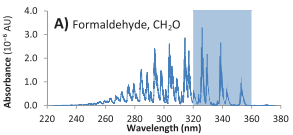
\includegraphics{Figures/HCHO/HCHOAbsorbanceDavenport.png}
      \caption{ HCHO spectrum, with a typical band of wavelengths used for DOAS path measurements.
	This is a portion of an image from \citet{Davenport2015}.}
      \label{ch_LitRev:fig:HCHOSpectrum}
    \end{figure}
    
    
    In MAX-DOAS retrievals, the measurements of light absorption are performed over several elevations in order to add some vertical resolution to the measurement of trace gas concentrations.
    An example of this is shown in figure \ref{ch_LitRev:fig:MAXDOASExample}, which was taken from \citet{Lee2015}.
    Recently MAX-DOAS has been used to examine HCHO profiles in the clean free troposphere \citep{Franco2015, Schreier2016} as well as in polluted city air \citep{Lee2015}.
    Depending on orography and atmospheric composition (ie. the influence of interfering chemicals), MAX-DOAS can be used to split the tropospheric column into two partial columns; giving a small amount of vertical resolution to HCHO measurements \citep[eg.]{Franco2015, Lee2015}.
    
    \begin{figure}
      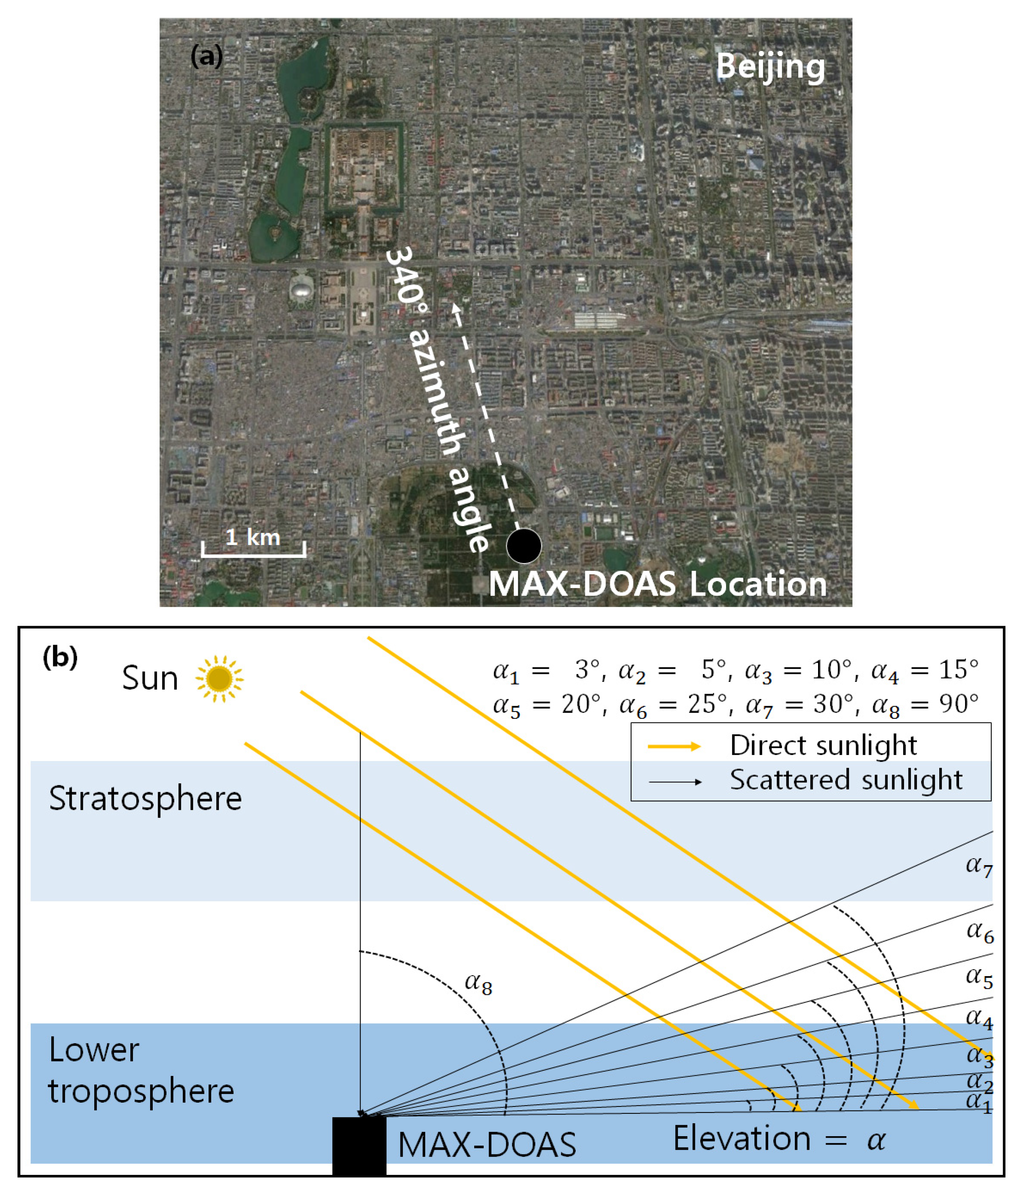
\includegraphics{Figures/MAXDoasExample.png}
      \caption{ %
        Image from \citet{Lee2015}.
      }
      \label{ch_LitRev:fig:MAXDOASExample}
    \end{figure}
    
    Other measurement techniques include chromatographic and fluorimetric methods, both of which differ widely from eachother and the spectroscopic method TODO: read \citep{Hak2005}).
    This resulted in HCHO not having a consistent network for global measurements like those for GHGs or Ozone \citep{FortemsCheiney2012}.
    
  \subsection{Relationship with glyoxyl and isoprene}
    Glyoxyl (CHOCHO) is important to us as it shares many properties with HCHO, and may provide additional information in determining isoprene emissions.
    Glyoxyl is another product of VOC oxidation in the atmosphere, with isoprene being the main source globally.
    Isoprene has been used to estimate isoprene emissions (see section \ref{ch_LitRev:sec:IsopFromHCHO}) but many uncertainties exist.
    One of these uncertainties is the yield of HCHO from isoprene, especially in low NO$_X$ environments.
    Glyoxyl could prove complementary to HCHO in constraining isoprene emissions (TODO: Read and cite Vrekoussis2009,2010, Chan Miller 2014, Alvarado 2014).
    
    Under high NO$_X$ conditions, glyoxyl forms rapidly, similarly to HCHO.
    However, glyoxyl also forms in low NO$_X$ environments both slowly (through isoprene epoxydiols), and rapidly (through di-hydroperoxide dicarbonyl compound photolysation (todo: read abstract and cite crounse(Autoxidation of Organic Compounds in the Atmosphere) 2013).
    This process is similar to the proposed mechanisms for hydroperoxyaldehydes by \citet{Peeters2014} and carbonyl nitrates (todo: read and cite M$\:{u}$ller 2014).
    
  \subsection{Satellite measurements}
    Satellite measurements of HCHO are relatively uncertain, however this can be improved by averaging over larger grid boxes or longer time scales.
    an example of this can be seen in \citet{Dufour2009}, where monthly averaging is used to decrease the measurements uncertainty.
    They examine HCHO in Europe, which is low; near the detection limit of satellite measurements.
    Taking monthly averages allows enough certainty that useful inversions can be determined to estimate the source emissions of HCHO.
    
    In satellite HCHO products, concentrations over the remote pacific ocean are sometimes used to analyse faulty instrument readings.
    This is due to the expected invariance of HCHO over this region.
    For instance GOME (an instrument which measures trace gases on board the ERS-2) corrects for an instrument artifact using modelled HCHO over the remote pacific \citep{Shim2015}.
    OMI HCHO products use a similar technique to account for sensor plate drift and changing bromine sensitivity \citep{Abad2015}
    
    For many places the tropospheric column HCHO measured by satellite is biased low, \citet{Zhu2016} examine six available datasets and show a bias of 20 - 51\% over south east USA when compared against a campaign of aircraft observations (SEAC$^4$RS).
    \citet{DeSmedt2015} also found a low bias from 20 - 40\% when comparing OMI and GOME2 observations against ground based vertical profiles, and \citet{Barkley2013} determine OMI to be 37\% low compared with aircraft measurements over Guyana.
    These bias can be corrected by improving the assumed apriori HCHO profiles which are used to calculate the AMFs of the satellite columns.
    
    The OMI measurements used in this research are recalculated using an updated estimate of HCHO profiles and validated against Wollongong total column measurements. 
    Similar to validation performed by other studies TODO: cite and exemplify a few studies ie: \citet{Zhu2016, Marais2015, Palmer2003} 
    
    Uncertainty in the OMI satellite instrument is calculated by the Smithsonian Astrophysical Observatory (SAO) group using the uncertainty in backscattered radiation retrievals \citep{Abad2015, Abad2016}.
    Another method of calculating the uncertainty is used by the Belgian Institute for Space Aeronomy (BIRA) group, who determine uncertainty from the standard deviation of HCHO over the remote pacific ocean (TODO: use both these methods for HCHO section)\citep{DeSmedt2012, DeSmedt2015}.
    
    GOME suffers from similar uncertainties to OMI, as the same general method of DOAS remote measurements are performed.
    The uncertainty from slant column fitting has been calculated for GOME to be $4\times10^{15}$ molecules cm$^{-2}$ \citep{Chance2000, Millet2006}. 
    The conversion factor for slant to vertical columns (AMF) calculation also suffers from errors; primarily from surface albedo, HCHO vertical profile apriori, aerosol, and cloud influence \citep{Millet2006}. 
    AMF uncertainties for GOME are calculated to be $1$ to $1.3\times10^{15}$ molecules cm$^{-2}$ by \citet{Shim2005}.
%----------------------------------------------------------------------------------------
%	Isoprene Section
%----------------------------------------------------------------------------------------
\section{Isoprene}
\label{ch_LitRev:sec:isoprene}

  \subsection{Basics}
    Isoprene, or 2-methylbuta-1,3-diene, is a Volatile Organic Compound (VOC) and has chemical formula of C$_5$H$_8$. 
    Isoprene effects NO$_X$ and HO$_Y$ cycling, and in the presence of NO$_X$, forms tropospheric ozone and SOAs \citep{Wagner2002, Millet2006}.
    Bottom up inventories of VOCs remain largely uncertain due to extensive extrapolation over plant functional types, changing land cover, and parameterised environmental stressors (todo: read and \citep{Guenther2000}).

  \subsection{Sources and Sinks}
    Methane and isoprene each comprise around a third of the yearly global total emission of VOCs.
    However, methane is relatively long lived (years) and is well mixed in the atmosphere while isoprene levels are very volatile and spatially diverse due to a life time of around an hour.
    Estimates put global isoprene emission at roughly 600 Tg yr$^{-1}$, emitted mostly during the day.
    Major emitters are tropical broadleafs (notably eucalypts), and scrubs \citep{Guenther2006, Arneth2008, Niinemets2010, Monks2015}.
    
    Isoprene has a short lifetime during the day, roughly an hour due to OH oxidation (todo: abstract and cite Atkinson and Arey 2003\citep{AtkinsonArey2003}).
    At night when OH concentrations have dropped, isoprene can remain in the atmosphere to be transported. 
    Typically less than half of this night time isoprene is removed through ozonolysis \citep{AtkinsonArey2003}, however, in polluted areas where high levels of NO$_X$ exist, isoprene is consumed by a different radical.
    During the night time, nitrate radicals (NO$_3$) build up, especially in areas with high NO$_X$ levels.
    In areas with high NO$_X$ levels, greater than 20\% of the isoprene emitted late in the day ends up being oxidised by the NO$_3$ radical over night \citep{Brown2009}.
    So while night time isoprene is not as highly concentrated, is does have varying biogenic and anthropogenic sinks.
    At night isoprene has affects on both NO$_X$ concentrations and ozone levels, and can form harmful SOAs \citep{Brown2009, Mao2013}.

    The oxidation products of isoprene and O$_2$ produce various isomers of isoprene hydroxyperoxy radicals (ISOPO$_2$), along with MACR and MVK. 
    The ISOPO$_2$ radicals are eventually destroyed by NO, HO$_2$ and other RO$_2$, with most pathways potentially producing HCHO \citep{Wolf2016}.
    
    Isoprene oxidation by OH is less well understood when lower concentrations of NO are present in the atmosphere.
    Initially isoprene was thought to be a sink for atmospheric oxidants \citep[eg.]{Guenther2000}.
    It was thought that in low NO environments, like those far from anthropogenic pollution and fires, oxidation of isoprene would create hydroxyhydroperoxides (ISOPOOH) and lead to low concentrations of OH and HO$_2$ (together known as HO$_X$) \citet{Paulot2009b}.
    In \citet{Paulot2009b}, the HO$_X$ levels are shown to be largely unnaffected by isoprene concentrations.
    They show that ISOPOOH is formed in yields $> 70\%$, and MACR and MVK is formed with yields $< 30\%$.
    The formation of MACR and MVK produces some HO$_X$, although not enough to close the gap.
    \citet{Paulot2009b} goes on to suggest (and provide experimental evidence) that dihydroxyperoxides (IEPOX) are formed from oxidation of the ISOPOOH, which form precursors for SOAs as well as closing the HO$_X$ concentration gap.
    They then use GEOS-Chem, modified to include IEPOX formation, to estimate that one third of isoprene peroxy radicals react with HO$_2$, and two thirds react with NO. 
    Their work showed another pathway for isoprene based SOA creation, and additionally estimated $95 \pm 45$~TgC yr$^{-1}$ IEPOX being created in the atmosphere without any inclusion in CTMs at that time.
    In \cite{Crounse2012}, MACR products are examined in various conditions and hydroxy recycling is also observed in low NO conditions. 
    
    Although understanding of OH production/recycling in these low NO conditions has been improved, many observations of OH are still quite under-predicted in models \citep{Mao2012}.
    It was shown in \citet{Mao2012}, for a remote forest in California, that the traditional method of OH measurement may be affected by instrument internally generated OH from VOC oxidation.
    This lends more credence to the current understanding of VOC oxidation as it closed the gap between measurements and model predictions.
  %\subsection{Products from isoprene}
  \subsection{Factors affecting isoprene emissions}
    
    \citet{Marais2014} examine factors affecting isoprene emissions, showing how emissions are sensitive to various environmental factors.
    Their work used MEGAN \citep{Guenther1995} and GEOS-Chem to look at how these factors affect surface ozone and particulate matter in Africa.
    One of the important uncertainties seen in MEGAN within this work is the isoprene emissions due to plant type. 
    Canopy level isoprene measurements are made using relaxed eddy accumulation (REA) at several sites in Africa.
    One plant type near a measurement site emits more than other species and it's actual distribution on a larger scale is completely unknown - leading to possible overestimations in MEGAN.
    Current emissions estimates require more validation against observations, and recently a comparison of two major VOC models (MEGAN and ORCHIDEE) was undertaken by \cite{Messina2016} reiterating this requirement.
    In their work they examine model sensitivities and show that the important parameters are leaf area index (LAI), emission factors (EF), plant functional type (PFT), and light density fraction (LDF).
    There is high uncertainty in LAI and EF, which require more or improved measurements at the global scale.
    LDF paramterisation needs improvement and these models require more PFTs.  
    
    \citet{Stavrakou2014} examined modelled Asian emissions and altered model parameters for temperature, plant type emission factors, incoming solar radiation (insolation) intensity, land use changes, and palm tree forest expansion.
    Changes were constrained by a network of radiation measurements and some experiments with south east Asian forest emissions - and led to reduction in isoprene emissions by a factor of two over the region.
    The Asian region is also shown to have a strong correlation with the Oceanic Niño Index (ONI), with positive anomalies associated with El Niño.
  
  \subsection{Estimates}
  \label{ch_LitRev:sec:BVOCestimates}
    It used to be thought that anthropogenic and biogenic emissions of VOCs were roughly similar (TODO abstract of \citep{Mueller1992}, and more cites).
    It's now clear that biogenic isoprene emissions are far greater than anthropogenic emissions of VOCs \citep{Guenther2006, Kefauver2014}. 
    The estimates are still fairly uncertain, as global measurements are difficult and regional emissions can be very different. 
    The lack of accuracy in BVOC emissions estimates has a large effect on determining with confidence the sources and distribution of pollutants including ozone and organic aerosols.
    Accuracy in VOC measurements is important: it has been shown that even the diurnal pattern of isoprene emissions has an effect on modelling ground level ozone \citep{Hewitt2011,Fan2004}.
    These uncertainties could explain why models of HCHO over Australia are poor at reproducing satellite measurements \citep{Stavrakou2009}.

    \citet{Guenther2006} estimates that the Australian outback is among the world's strongest isoprene emitters with forests in SE Australia having emission factors greater than 16 mg m$^{-2}$ h$^{-1}$ (see figure \ref{ch_LitRev:fig:meganisoprene}).
    These emissions factor estimates are not well verified as there is little coverage of isoprene (or other BVOC) emissions measurements over Australia.
    However, comprehensive coverage of one high yield (generally) product in the atmosphere over Australia exists in the form of satellite measurements.
    
    It is important to note that many estimates of isoprene emission are based on a few algorithms of isoprene emission which can depend greatly on input parameters \citep{Niinemets2010}.
    \citet{Yue2015} has shown that this is still a problem by looking at land carbon fluxes and modelling the sensitivity to VOC emissions estimates using two independent models of VOC emission.
    One model is photosynthesis based and estimates isoprene emissions using electron transfer energies and leaf physiology \citep{Niinemets1999}, while the other (MEGAN) uses the light and canopy temperature (\citep{Guenther1995} TODO: Arneth et al., 2007; Unger et al., 2013).
    Both are sensitive to light and temperature parameterisations.
    
    
    \begin{figure}
      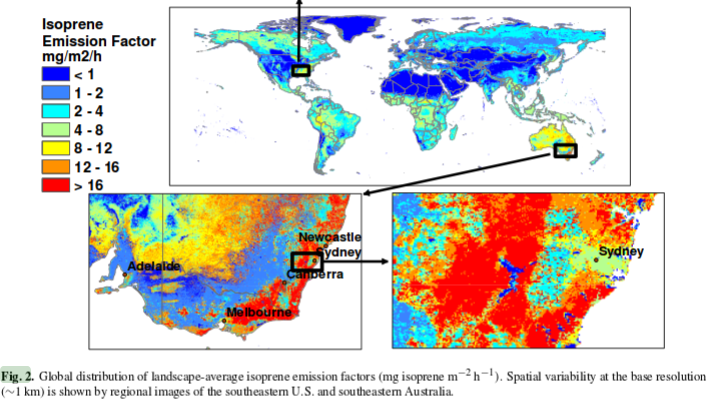
\includegraphics{Figures/MeganIsoprene1.png}
      \caption{ Part of a figure from \citet{Guenther2006} showing global isoprene emission factors. }
      \label{ch_LitRev:fig:meganisoprene}
    \end{figure}
    
  \subsection{Isoprene to HCHO}
    \label{ch_LitRev:sec:IsopFromHCHO}
    In the remote troposphere HCHO production is dominated by methane oxidation, while in the continental boundary layer (CBL) production is largely due to NMVOCs \citep{Abbot2003, Kefauver2014}.
    NMVOCs are alkanes, alkenes, aromatic hydrocarbons and isoprene.
    Isoprene is hard to measure directly due to its short lifetime and weak spectral absorption, instead formaldehyde is often used as a proxy \citep{Millet2006, Dufour2009, Marais2012, bauwens2013satellite, Kefauver2014, Bauwens2016}.
    Formaldehyde formed in the troposphere is mostly due to VOC (roughly one third each: methane, isoprene, others) oxidation.
    We can model this oxidation process in order to work out how much VOC is present based on the total HCHO.
    This requires among other things an idea of which VOCs are present and their yields of HCHO.
    
    The method used to develop top-down isoprene inference using satellites was developed initially by \citet{Palmer2001, Palmer2003}. 
    Isoprene emissions fluxes were derived using the Global Ozone Monitoring Experiment (GOME) satellite instrument.
    Palmer's method improved biogenic isoprene emissions estimates (compared with in-situ measurements) over two available inventories: the U.S. EPA Biogenic Emssions Inventory System (BEIS2) and the Global Emissions Inventory Activity (GEIA).
    This showed an inversion technique which could be used to improve large scale emissions estimates without further expensive measurement campaigns.
    
    \citet{Dufour2009} use HCHO from SCIAMACHY, and examine Europe using CHIMERE as the chemical model. 
    In their work they show that satellite measurements can reduce source emission uncertainty by a factor of two, where emissions are relatively large.
    
    Satellites recording reflected solar spectra use Differential Optical Absorption Spectroscopy (DOAS) to measure various trace gases in the atmosphere, including formaldehyde. 
    Formaldehyde levels in the continental boundary layer are generally dominated by chemical formation due to VOC (largely isoprene) emissions \citep{Kefauver2014}.
    While satellite measurements can only be used during daytime hours, HCHO lifetimes are sufficiently short that any nighttime will not affect midday observations \citep{Wolfe2016}.
    
    Satellites can be used to measure the seasonal and interannual variability of HCHO over Australia.
    These records can be compared with modeled estimates of HCHO and used as a proxy to estimate isoprene emissions.
    This has been done in North America \citep{Palmer2003, Millet2006}, South America, Africa, China, Europe \citep{Dufour2009}, and recently globally \citep{FortemsCheiney2012, Bauwens2016}.
    Often these works use two forms of measurement such as satellite and aircraft data combined for validation \citep{Marais2014}.
    
    Initially studies assumed a simple linear steady-state relationship between HCHO and it's precursors \citep{Palmer2003, Palmer2006, Millet2006}.
    This allowed a simple calculation of isoprene using the measured HCHO, with estimated reaction rates and yields.
    The methodology for calculating VOCs from HCHO is laid out in \citet{Palmer2003}, and takes into account the expected lifetime and reaction rates of the precursor VOCs and HCHO.
    Assuming HCHO is produced quickly from short-lived intermediates, and the column is at steady state:
    \begin{eqnarray*}
    VOC_i \overset{k_i}{\rightarrow} Y_i HCHO
    \end{eqnarray*}
    Where $Y_i$ is HCHO yield per C atom (a measure of how much HCHO will form per gram of C from a VOC within a system), and $k_i$ is the reaction rate.
    Then assuming a steady state of atmospheric HCHO ($\Omega$ molecules $cm^{-2}$) produced by oxidation of VOCs (VOC$_i$) and no horizontal transport:
    \begin{eqnarray*}
    \Omega = \frac{1}{k_{HCHO}} \sum_{i} Y_i E_i
    \end{eqnarray*}
    Where i indexes a chemical species, $k_{HCHO}$ is the HCHO loss rate due to OH and photolysis, Y$_i$ is the molar HCHO yield from oxidation of i, and $E_i$ is emission fluxes ( C atoms $cm^{-2}s^{-1}$).
    
    Estimates of Y$_i$ can be attained from a model as shown in \citet{Millet2006}.
    This involves a reduced major axis (RMA) correllation calculation between modelled HCHO and isoprene columns, multiplied by their loss rates (to photolysis and oxidation) (as a normalising factor).  
    In high NOx environments where HCHO has a lifetime on the order of 30 minutes, it can be used to map isoprene emissions with spatial resolution from 10-100 kms.
    Horizontal transport 'smears' the HCHO signal so that source location would need to be calculated using windspeeds and loss rates \citep{Palmer2001,Palmer2003}.
    For more details on this see section \ref{ch_LitRev:sec:smearing}.
    
    Another method of correcting isoprene emissions using observed HCHO total column involves a Bayesian inversion.
    \citet{Shim2005} work with GOME HCHO observations and GEOS-Chem, looking at areas with high signal to noise ratio (higher HCHO concentrations).
    They show that the model underestimates isoprene emissions and HCHO concentrations by 14-46\%, with the corrected VOC emissions reducing the model biases to 3-25\%.
    
    The Bayesian inversion is also used in \citet{Curci2010}, where a regional CTM (CHIMERE) simulates HCHO, which is compared against OMI observed HCHO and shown to be regionally biased.
    This bias is expected to be caused by errors in MEGAN's natural isoprene emissions.
    The CHIMERE model is used to derive yields of HCHO from the various local VOCs and these are then used in estimating local emissions.
    The model is run initially with emissions of BVOCs and reactive anthropogenic VOCs (RAVOCs) turned off in order to work out the background (b) values of these compounds.
    The Bayesian inversion is used to correct regionally biased biogenic isoprene emissions by optimising these parameters in order to simulate HCHO closest to the observed HCHO levels.
    \cite{Curci2010} uses CHIMERE as the forward model to determine the relationship between HCHO (y), isorene and reactive anthropogenic VOCs (\textbf{x}), using 
    \begin{equation}
        y=\mathbf{K}x + b + \epsilon
    \end{equation}
    where $\epsilon$ are the (assumed) independent errors in measurements.
    K is the Jacobian matrix determined from CHIMERE representing the sensitivity of y to the state variable x.
    This K matrix is used in conjunction with error covariance in x to determine the Maximum A Posteriori (MAP) solution to calculate the optimal estimate of x ($\hat{x}$).
    
    TODO: Read through this list of sources on the hcho to isop process : taken from Wolfe2015
    Such techniques have informed isoprene emission inventories in North America (Abbot et al., 2003; Millet et al., 2008 \citep{Palmer2003,Millet2006,Palmer2006}), South America (\citep{Barkley2013}, 2008), Europe \citep{Curci2010,Dufour2009}, Africa \citep{Marais2012}, Asia (Fu et al., 2007; Stavrakou et al., 2014), and globally (Fortems-Cheiney et al., 2012; \citep{Shim2005}; Stavrakou et al., 2009).
    
    More recently, full inversions that better account for transport, source attribution, and chemical schemes have been implemented \citep{FortemsCheiney2012}.
    TODO: full description of this better inversion technique going through FortemsCheiney2012.
  
  \subsection{Smearing}
  \label{ch_LitRev:sec:smearing}
    The distance travelled downwind (L$_{d,i}$ by a precursor (i) before becoming HCHO can be estimated using:
    \begin{equation*}
      L_{d,i} = \frac{U}{k_i - k_{HCHO}} \ln{ \left( \frac{k_i}{k_{HCHO}} \right) }
    \end{equation*}
    where U is windspeed.
    \citet{Palmer2003} further define a smearing length scale: L$_{s,i}$ as the distance downwind where a fraction (1 - $1/e$) of the precursor is completely transformed into HCHO.
    This equation uses the initial VOC column concentration ($[VOC]_0$) at the point of emission and mass balance equations, and is as follows:
    \begin{equation}
      \frac{1}{k_{HCHO}-k_i} \left( k_{HCHO} \exp{ \left[ \frac{-k_i L_{s,i}}{U} \right]} -k_i \exp{ \left[ \frac{-k_{HCHO} L_{s,i}}{U} \right]} \right) = \frac{1}{e} 
    \end{equation}
    with limiting values L$_{s,i} \rightarrow U/k_i$ for $k_i << k_{HCHO}$, and L$_{s,i} \rightarrow U/k_{HCHO}$ for $k_{HCHO} << k_i$.  
    
    Accounting for transport of the precursors is important, especially in low NO$_X$ conditions in which isoprene has a longer lifetime (days).
    This allows horizontal transport to occur and complicates the algorithms, as can be seen by the smearing length scale which increases beyond the 100~km.
    For conditions where VOCs have a lifetime of days determining the major HCHO contributors requires a complex inversion to map HCHO columns to VOC emissions.
    
  \subsection{Measurements}
  
    There are relatively few measurements of isoprene in the southern hemisphere, including MUMBA(TODO CITE), other campaigns?, and very recently that girl from Macquarie University with an instrument in the daintree rainforest(TODO CITE, DESCRIBE?).
    Since 1997, when GOME first measured HCHO over Asia (TODO cite thomas 1998), satellites have been able to provide a total column measurement of one of the primary products of isoprene.
    
    
  \subsection{Estimates}
    There are two commonly used ways of estimating isoprene emissions, top-down or bottom-up.
    Bottom-up emission estimates generally model the flora and events which emit isoprene, like Eucalypts, factories, shrubs, leaf areas under sunlight, etc.
    Understanding how much isoprene is emitted, when and by what is more complicated than it sounds, and since little data exists with which to verify these bottom-up emission inventories they are uncertain on a large scale.
    Top-down estimates look at how much of a chemical is in the atmosphere and try to work out how much of it's major precursors were emitted.
    For isoprene this is done by looking at atmospheric HCHO enhancement, which can be largely attributed to isoprene emissions as long NO$_X$ and transport effects are accounted for.
  
  \subsection{Isoprene products}
    Isoprene forms many products with various lifetimes, here I will present an overview of some important mechanisms which affect oxidation capacity, ozone and aerosol production.
    Isoprene reacts with OH leading to peroxy radical (ISOPO$_2$) formation.
    In the presence of NO$_X$ ISOPO$_2$ forms organic nitrates after reacting with NO.
    These affect levels of both HO$_X$ (H, OH, peroxy radicals) and NO$_X$, acting as a sink (\citet{Mao2013} and references therein).
    
    The first generation of organic nitrates produced by isoprene oxidation range from 7\% to 12\%, shown in laboratory experiments (todo read abstracts and cite papers in the 3rd paragraph of intro to Mao2013),
    A portion of isoprene nitrates are recycled back to NO$_X$, so may serve as a reservoir of nitrogen and allow its transport to the boundary layer of remote regions (TODO: as prior todo).
    
    During the night isoprene is oxidised by NO$_3$ radicals, which joins to one of the double bonds and produces organic nitrates in high yield (65\% to 85\%) \citep{Mao2013}. (todo: read mao2013 para 3 cites for)
    These organic nitrates go on to produce further SOAs \citep{Rollins2009} (todo read Rollins2009).
  
    Todo: More on \citep{Mao2013} ()chemistry mechanism used in GEOS-Chem v9.02)
    For specific information on the isoprene oxidation mechanisms used by GEOS-Chem V10-01 (used in this work), see section \ref{ch_isop:sec:GEOSChemMechanisms}.
  
  \subsection{Radiative Forcing}

    
%----------------------------------------------------------------------------------------
%	SECTION 5
%----------------------------------------------------------------------------------------
\section{Dust}
\label{ch_LitRev:sec:dust}

  Australia is the greatest source of dust in the southern hemisphere producing around 120~Tg yr$^{-1}$ \citep{Li2008}, however model validation and analysis over Australia is relatively scarce with more focus applied to the northern hemisphere \citep{Fairlie2007, Ridley2013}.
  Atmospheric dust has many direct effects including reduced surface insolation, mineral transfer to remote ocean regions, and health degradation in populated areas \citep{Shao2007}.
  Direct and indirect effects of dust have many implications which are not fully understood, with many models still struggling to explain the atmospheric cycling of dust at larger scales \citep{Rotstayn2011}.

  Australian dust emissions involve various weather conditions, convolving the ENSO cycle with flooding, droughts, and winds.
  Rivers and rain build up the particulate matter in many areas, these are referred to as fluvial deposits.
  Fluvial deposits in the Eyre basin increase the dust base load, which will only have mobility during suitable dry weather conditions.
  These deposits are saltated (loosened from the surface) and transported by strong winds\citep{Zender2003}.

  Synoptic scale measurements of dust concentrations in Australia are made by the Bureau of Meteorology (BOM) and can be used to estimate dust transport caused by large storms. 
  Single storms have been estimated to move up to 2.5 Tg of dust off shore in a single day.
  Yearly dust emissions in Australia are somewhere between 10 and 110 Tg yr$^{-1}$.
  These estimates exemplify the large variability in Australian annual dust transport.

  Dust plays a large role in the oceanic carbon cycle, as dust is a major source of oceanic iron (Fe) deposition.
  Some regions in the ocean are high in nutrients, but low in chlorophyll (HNLC), due to a lack of Fe.
  Oceanic carbon cycling is a complex system in which Fe is a limiting factor, required by plankton in order to fix atmospheric nitrogen into a more bioavailable form such as ammonia.
  Atmospheric deposition into the oceans is a very poorly constrained variable in global models \citep{Grand2015}.
  Model estimates of trace element oceanic deposition are required to quantify the atmospheric impact due to a dearth of in situ measurements in remote open ocean regions.

  Measurements of dissolved iron (DFe) at very low concentrations like those found in surface ocean waters are very easily contaminated, which has contributed the the fragmentary and scarce nature of DFe ocean data sets \citep{Rijkenberg2014}.
  Recent analysis of the US Climate Variability and Predictability (CLIVAR)-CO$_{2}$ Repeat Hydrography Program predicted total deposition flux with uncertainty at a factor of 3.5 \citep{Grand2015}.
  Some headway has been made with the recent GEOTRACES program which has several transects of the major oceans and measures trace elements over multiple depths including Al, Ba, Cu, Cd, Fe, Mn, Ni, Pb, and Zn.
    
  Total iron (TFe) emissions from dust and combustion sources are estimated (by average of several global models) at approximately 35~Tg yr$^{-1}$ and 2 Tg yr$^{-1}$ respectively. A two fold increase in Fe dissolution may have occurred since 1850 due to increased anthropogenic emissions and atmospheric acidity.
  This increase may revert by 2100 due to the affects of emission regulations \citep{Myriokefalitakis2015}.
  Dust, TFe and DFe have strong temporally and spatial variability, with changes having most impact upon HnLC regions.

  Another environmental impact of dust is its contribution to fine particulate matter in the atmosphere.
  Several studies have shown that long term exposure to fine particulate matter (PM2.5) increases mortality. 
  Estimates of yearly premature deaths related to PM2.5 are $\sim$ 2-3 million \citep{Hoek2013, Krewski2009, Silva2013, Lelieveld2015}.   
  These estimates are made using global atmospheric models or model ensembles to quantify population exposure before applying epidemiological models to estimate the increased death rates.
  The main source of uncertainty in premature death rates arises from the difference and uncertainties between and within the atmospheric models.

  Dust affects global climate change through direct radiative forcing.
  Uncertainties in the atmospheric dust concentrations make accurate determination of radiative forcing from other sources more difficult \citep{IPCC_2013_chap8}.


%----------------------------------------------------------------------------------------
%	SECTION 6
%----------------------------------------------------------------------------------------
\section{Models}
\label{ch_LitRev:sec:models}

  \subsection{Chemical Transport Models}
  
    Chemical Transport Models (CTMs) simulate production, loss, and transport of chemical species.
    This is generally calculated using one or both of the Eulerian (box) or Lagrangian (puff) frames of reference.
    CTMs normally solve the continuity equations simultaneously with chemical production and loss for chemicals under inspection. 
    The continuity equations describe transport of a conserved quantity such as mass, which, solved together with production and loss of a chemical forms the basis for a CTM.
    This basis enables a record of the chemical densities and transport over time as a model runs.
    The general continuity equation links a quantity of a substance (q) to the field in which it flows and can be described by the formula:
    \begin{eqnarray*}
	\frac{\partial \rho}{\partial t} + \nabla \cdot j &=& \sigma 
    \end{eqnarray*}
    where $\rho$ is density of q in the field, t is time, $\nabla$ is divergence, j is the flux (the amount of q per unit area per unit time entering or leaving the field), and $\sigma$ is the generation of q per unit volume per unit time.
    Note that $\sigma$ can be positive or negative due to sources and sinks.

    The type of model best suited to modelling the entire earth uses the Eulerian frame of reference, where the atmosphere is broken up into 3-D boxes with densities and transport calculated and stored for arbitrary sequential steps in time at each location.
    The mass balance equation must be satisfied in any realistic long term box model and is as follows: 
    \begin{align*}
	\frac{dm}{dt} &=& \sum{sources}-\sum{sinks} \\
	&=& F_{in} + E + P - F_{out} - L - D 
    \end{align*}
    where m is mass of a chemical, E and D are emission and deposition, P and L are production and loss, and F is chemical transport in and out, as shown in figure \ref{ch_LitRev:fig:boxmodel}.
    Many chemical species interact with each other through production and loss. 
    Any large chemical model will solve this mass balance equation over highly coupled arrays of partial differential equations which can be complex and time consuming.

    In many CTMs the isoprene emissions are calculated elsewhere with their own models (EG: \citet{Guenther2006}).
    These estimates can then be used as boundary conditions.
    Trace gases with short lifetimes and complex chemistry such as isoprene are often hard to measure which makes verifying model estimates difficult.

    \begin{figure}
      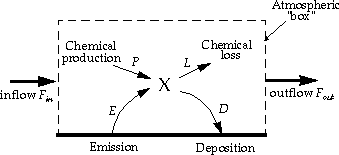
\includegraphics{Figures/boxmodel.png}
      \caption{ Standard box model parameters, image taken from \citet{Jacob_1999_book}. }
      \label{ch_LitRev:fig:boxmodel}
    \end{figure}

  \subsection{GEOS-Chem}
  
    GEOS-Chem is a well supported global, Eulerian CTM with a state of the science chemical mechanism, with transport driven by meteorological input from the Goddard Earth Observing System (GEOS) of the NASA Global Modeling and Assimilation Office (GMAO).
    GEOS-Chem simulates more than 100 chemical species from the earth's surface up to the edge of space (0.01 hPa) and can be used in combination with remote and in-situ sensing data to give a verifiable estimate of atmospheric gases and aerosols.
    It was developed, and is maintained, by Harvard University staff as well as users and researchers worldwide. 
    Several driving meteorological fields exist with different resolutions, the finest at 0.25 by 0.3125$^\circ$ horizontally at 5 minute time steps with 72 vertical levels.
    
   GEOS-Chem has boundary conditions based on several meteorological and emissions inventories, the following are the versions of theses used by GEOS-Chem v 10.01. 
   Meteorological fields can be driven by NASA's GEOS-5 data (0.5$^{\circ}$ x 0.666$^{\circ}$) (TODO:Chen et al., 2009), which exists up to 2013, or GEOS-FP data (0.25$^{\circ}$ x 0.3125$^{\circ}$).
   Fire emissions come from the GFED4 product \citep{Giglio2013}. Anthropogenic VOC emissions come from the EDGAR inventory, while biogenic VOC emissions are coupled to the MEGAN model TODO:cites.
   The estimated biogenic VOC emissions are important to the work done in this thesis and are discussed in somewhat more detail in section \ref{ch_LitRev:sec:BVOCestimates}.

    Combining satellite data with model outcomes provides a platform for the understanding of natural processes to be tested now and into the future over Australia and anywhere with few in-situ measurements.
    Due to the low availability of in-situ data covering most of the Australian continent, a combination of the models with satellite data may provide improved understanding of emissions from Australian landscapes.
    Improved emissions estimates will in turn improve the accuracy of CTMs, providing better predictions of atmospheric composition and its response to ongoing environmental change.
  
%----------------------------------------------------------------------------------------
%	SECTION 7
%----------------------------------------------------------------------------------------
\section{Satellites}
\label{ch_LitRev:sec:satellites}


  \subsection{Useful satellites}
    Several satellites provide long term trace gas observations with near complete global coverage, including the ERS-2 launched in April 1995 which houses the GOME ultraviolet and visible (UV-Vis) spectrometer, the AURA launched in July 2004 which houses the OMI UV-Vis spectrometer, the MetOp-A and B launched in October 2006 and September 2012 respectively both housing a GOME-2 UV-Vis spectrometer.
    These satellites are on Low Earth Orbit (LEO) trajectories and overpass any area up to once per day. 
    They record near nadir (nearly vertical) reflected spectra between around 250-700~nm split into spectral components at around $0.3$~nm in order to calculate trace gases including O$_3$, NO$_2$, and HCHO.
    An example of a spectrum retrieved from the GOME-2 instrument is given in figure \ref{ch_LitRev:fig:gomeproducts}.

    \begin{figure}
      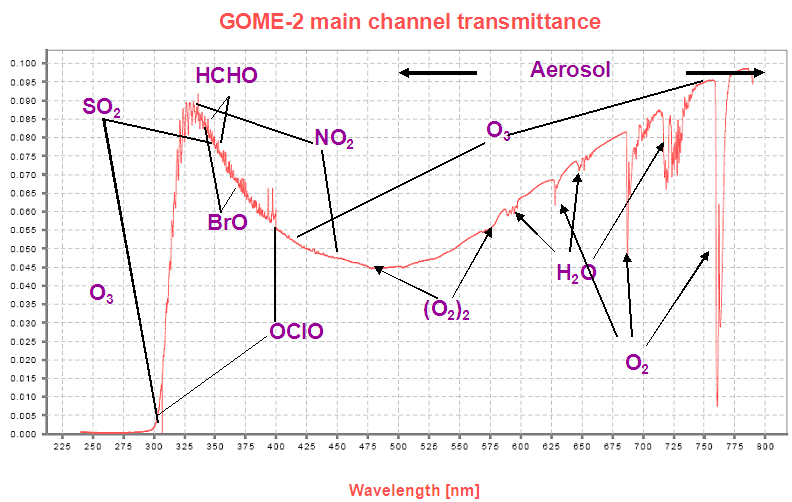
\includegraphics[width=\textwidth]{Figures/GOME_SPECTRUM.jpg}
      \caption{An example spectrum showing interferences used for species concentration measurements by GOME-2. Image by EUMETSAT and ESA \citep{GOME2Image}.}
      \label{ch_LitRev:fig:gomeproducts}
    \end{figure}

    The OMI instruement in particular is used within my work to calculate of HCHO, it records spectra from 264-504~nm using an array of 60 detectors with mid-resolution (0.4-0.6~nm).
    This band of wavelengths allows measurments of trace gases including O$_3$, NO$_2$, SO$_2$, HCHO, and various other quantities like surface UV radiation. 
    Recently \cite{Schenkeveld2017} analysed the performance over time of the instrument and found irradiance degradation of 3-8\%, changed radiances of 1-2\%, and a stable wavelength calibration within 0.005-0.020~nm.
    These changes are measured excluding the row anomaly effect, which is relatively stable since 2011, although it is still growing and remains the most serious concern.
    \cite{Schenkeveld2017} concludes that OMI data is still of high quality and will deliver useful information for 5-10 more years.
    
    Formaldehyde (HCHO) is often used as a proxy to estimate isoprene emissions \citep{Marais2012,bauwens2013satellite}.
    Satellites can use DOAS techniques with radiative transfer calculations on solar radiation absorption spectra to measure column HCHO (eg: \citet{Leue2001}).
    Several public data servers are available which include products from the satellites just mentioned, including NASA's Mirador (http://mirador.gsfc.nasa.gov/) and the Belgian Institute for Space Aeronomy (IASB-BIRA) Aeronomie site (http://h2co.aeronomie.be/).

    Instruments including MODIS on board the AQUA and TERRA satellites are able to determine aerosol optical depth (AOD), a measure of atmospheric scatter and absorbance. 
    An AOD of under 0.05 indicates a clear sky, while values of 1 or greater indicate increasingly hazy conditions.
    This is an important atmospheric property allowing us to track dust storms and pollution events as well as determine where measurements from other instruments may be compromised by high interference.
    Satellite measured AOD requires validation by more accurate ground based instruments like those of AERONET which uses more than 200 sun photometers scattered globally. 
  
  \subsection{Comparisons with Models}
  
    DOAS methods can be heavily influenced by the initial estimates of a trace gas profile (the apriori) which is often produced by modelling, so when comparing models of these trace gases to satellite measurements extra care needs to be taken to avoid introducing bias from unrealistic a priori assumptions.
    One way to remove these apriori influences is through the satellite's averaging kernal, which takes into account the vertical profile of the modelled trace gas and instrument sensitivity to the trace gas \citep{Eskes2003, Palmer2001}.
    Measurements done using DOAS often apply a forward radiative transfer model (RTM) such as LIDORT in order to determine a trace gas's radiative properties at various altitudes.
  
  \subsection{DOAS}
    TODO: some of this is repeated in isoprene chapter satellite section.
    
    The DOAS technique uses solar radiation absorption spectra to measure trace gases through paths of light.
    The RTM used in DOAS techniques is based on Beer's law relating the attenuation of light to the properties of the medium it travels through.
    Beer's law states that $ T = I/I_0 = e^{-\tau} $ with T being transmittance, $\tau$ being optical depth, and I, I$_0$ being radiant flux received at instrument and emitted at source respectively.
    Using 
    $ \tau_i = \int \rho_i \beta_i ds $ gives us:
    $$ I = I_0 \exp {\left( \Sigma_i \int \rho_i \beta_i ds \right) } $$
    Where i represents a chemical species index, $\rho$ is a species density(molecules per cm$^3$), $\beta$ is the scattering and absorption cross section area (cm$^2$), and the integral over ds represents integration over the path from light source to instrument.
    The forward RTM used for satellite data products also involves functions representing extinction from Mie and Rayleigh scattering, and the efficiency of these on intensities from the trace gas under inspection, as well as accounting for various atmospheric parameters which may or may not be estimated (e.g. albedo).
    
    To convert the trace gas profile from a reflected solar radiance column (slanted along the light path) into a purely vertical column requires calculations of an air mass factor (AMF).
    In satellite data, the AMF is typically a scalar value for each horizontal grid point which will equal the ratio of the total vertical column density to the total slant column density. This value should also account for instrument sensitivities to various wavelengths at various altitudes, and is unique for each trace gas under consideration.
  
